\documentclass[10pt]{article}
\usepackage{hyperref}
\usepackage{graphicx}
\usepackage{array}
\usepackage{fancyvrb}
\graphicspath{ {./} }
\hypersetup{
    colorlinks=true,
    linkcolor=blue,
    filecolor=magenta,      
    urlcolor=cyan,
}
\addtolength{\oddsidemargin}{-.875in}
	\addtolength{\evensidemargin}{-.875in}
	\addtolength{\textwidth}{1.75in}

	\addtolength{\topmargin}{-.875in}
	\addtolength{\textheight}{1.75in}
\renewcommand{\baselinestretch}{0.97}
\title{Project 1: 
PayRental - Property Renting Marketplace}

\author {Akshay Neema (2016CS10323), Riya Singh (2016CS50388), Siddhant Shingi (2016CS10310)}

\date{Due date: March 1, 2020, 11:55pm IST}

\begin{document}

\maketitle
\section{Description}
\subsection{Project Description}
Airbnb is an online-based marketing company that connects people looking for accommodation (Airbnb guests) to people looking to rent their properties (Airbnb hosts) on a short-term or long-term basis. As a rental ecosystem, Airbnb generates tons of data including but not limited to the density of rentals across regions (cities and neighborhoods), price variations across rentals, host-guest interactions in the form of reviews, and so forth. \newline
\newline
Our idea is to create PayRental, a property renting marketplace which allows the user to match with the hosts who have put up their properties on rent. We will perform an exploratory data analysis of the dataset to understand the rental landscape through various visualisations. The complete system is as follows :-
\begin{itemize}
    \item Allows users to create a \textit{secured user account} which opens the PayRental homescreen. Users can choose from the property listings based on metrics like price and location. Once, chosen there is an option for booking the property and a calendar which let's the users know the availability of the listings. 
    \item Allows the hosts to create a \textit{secured host account} which opens the PayRental homescreen. Hosts are given the option to check out their listings - the bookings, the availability etc. and add or remove listings. 
\end{itemize}

\subsection{Entities and Attributes}

\begin{table}[!htbp]
\begin{center}
 \begin{tabular}{||c c||} 
 \hline
 Entity & Attributes  \\ [0.5ex] 
 \hline\hline
 Property & id, name, property type, root type, price, city, latitude, longitude, min nights, max nights  \\ 
 \hline
 Reviews & id, date \\
 \hline
 Calender & date, available \\
 \hline
 Users & user id, name, password \\
 \hline
 Hosts & host id, name, password \\
  \hline
 Bookings & id, check-in date, check-out date, #adults, #children \\
 \hline
\end{tabular}
\caption {List of Entities and Attributes}
\end{center}
\end{table}
\vspace{-1cm}
\begin{table}[!htbp]
\begin{center}
 \begin{tabular}{|c |>{\centering\arraybackslash}m{40 em} |} 
 \hline
 Attribute & Permitted Values  \\ [0.5ex] 
 \hline\hline
 City & Chicago, New York, Los Angeles  \\ 
 \hline
 Room type & Entire home/apt, Private room, Shared room, Hotel room \\
 \hline
 Property type & Aparthotel, Apartment, Barn, Bed and breakfast, Boat, Boutique hotel, Bungalow, Bus, Cabin, Camper/RV, Campsite, Casa particular (Cuba), Castle, Cave, Chalet, Condohotel, Condominium, Cottage, Dome house, Dorm, Earth house, Farm stay, Guesthouse, Guest suite, Hostel, Hotel, House, Houseboat, Hut, Igloo, In-law, Island, Lighthouse, Loft, Minsu (Taiwan), Nature lodge, Other, Pension (South Korea), Plane, Resort, Serviced apartment, Tent, Timeshare, Tiny house, Tipi, Townhouse, Train, Treehouse, Vacation home, Villa \\
 \hline
 Dates & Jan, 2019 - Dec, 2019 
 \\
  \hline
\end{tabular}
\caption {Structure of downloaded raw data}
\end{center}
\end{table}

\pagebreak



\section{Data Source and Statistics}

\subsection{Data Source}
The data is taken from officially available \href{http://insideairbnb.com/get-the-data.html}{Airbnb dataset} curated in late 2019. The Airbnb data consists mainly of three tables :-
\newline
1. \textbf{Listings} : This table contains the information of all the property listings on the site of Airbnb, with 106 attributes some of which are \textit{price (double precision)}, \textit{listing type, host name, latitude, review per month, scores } and \textit{ratings}. 
\newline
2. \textbf{Reviews} : This table consists of the reviews given by the guests and has the following attributes - \textit{date, listing id, reviewer id} and\textit{ comment} \textit{(textual)}.
\newline
3. \textbf{Calendar} : Provide the detail of booking by each listing. It has the attributes - \textit{date, listing id, available} and \textit{price}. 
\newline
\begin{table}[!htbp]
\begin{center}
 \begin{tabular}{||c c c ||} 
 \hline
 Table Name & Number of Attributes & Key Attributes \\ [0.5ex] 
 \hline
 Listings &  106 & id, host id, price, review per month, is superhost, score \\ 
 \hline
 Reviews & 6 & listing id, id, date, reviewer id, reviewer name, comments \\
 \hline
 Calendar & 7 & listing id, date, available, price, min nights, max nights\\
 \hline
\end{tabular}
\caption {Structure of raw data}
\end{center}
\end{table}
\subsection{Data Retrieval and Cleanup}
Airbnb online data has property, review and calendar data for 120 cities all over the world. Out of these 120 cities, 28 cities are located in United States. We choose 3 most dense cities (w.r.t the Airbnb properties) in the United States due to extremely large size restrictions especially on strings like comment. No scraping was required as the data is available in .csv format. 
\newline
Mainly the cleanup was done manually by discarding the redundant or unnecessary columns). Further all the '\text{\textbar}' characters in string type columns were replaced by ',' and '\text{\textbar}' was set as delimeter in the csv files. After the cleanup, data was inserted to the table using bulk copy. 
\newline 
After the cleanup the attributes and the tables are :-
\newline
\begin{enumerate}
    \item \textbf{Table: payrental} 
    \newline
    city\_data , state\_data , id , listing\_url , scrape\_id , last\_scraped , name , summary , space , experiences\_offered, neighborhood\_overview , notes , transit , access , interaction , house\_rules , thumbnail\_url , medium\_url , picture\_url , xl\_picture\_url , host\_id , host\_name , host\_since , host\_location , host\_about , host\_response\_time, host\_response\_rate , host\_acceptance\_rate , host\_is\_superhost , host\_listings\_count , host\_identity\_verified, street , neighbourhood , neighbourhood\_cleansed , neighbourhood\_group\_cleansed , city , state , zipcode , market , smart\_location , country\_code , country , latitude , longitude , is\_location\_exact , property\_type , room\_type , accommodates , bathrooms , bedrooms , beds , amenities , square\_feet , price, weekly\_price , monthly\_price , security\_deposit , cleaning\_fee , guests\_included , extra\_people , minimum\_nights , maximum\_nights , has\_availability , availability\_30 , availability\_60 , availability\_90 , availability\_365 and so on.
    \item  \textbf{Table: reviews} 
    \newline
    city , state , listing\_id , id , date , reviewer\_id
    \item  \textbf{Table: calender} 
    \newline
    city , state , listing\_id , date , available , price , adjusted\_price , minimum\_nights , maximum\_nights
    \item \textbf{Table: users} 
    \newline
    user\_id , name , username , password
    \item \textbf{Table: hosts} 
    \newline
    host\_id , host\_name , host\_username , password
    \item  \textbf{Table: bookings} 
    \newline
    booking\_id , property\_id , host\_id , user\_id , check\_in\_date , check\_out\_date , number\_adults , number\_children
\end{enumerate}

\subsection{Statistics}
\begin{table}[!htbp]
\begin{center}
 \begin{tabular}{||c c c c||} 
 \hline
 Table Name & Table Size & No.of Tuples & Time to Load \\ [0.5ex] 
 \hline
Calender    & 266 MB       &    3078751  &  11116.739 ms  \\ 
 \hline
Reviews     & 217 MB        &    2974950  &  26839.228 ms \\
 \hline
 Payrental   & 170 MB       &      98259    &  51242.337 ms\\
 \hline
 Users         & 132 MB       &    2423928  &  3764.284 ms\\
 \hline
 Hosts         & 3952 kB      &      65356     &  176.990 ms\\
 \hline
\end{tabular}
\caption {Data Statistics}
\end{center}
\end{table}

We have chosen three cities for a close exploratory data analysis from the Airbnb data. The cities were chosen on the basis of popularity and usage of Airbnb in and with a reasonable number of listings. The cities are \textbf{New York, Los Angeles and Chicago} and we will mostly be analysing the given data of these cities. 

\begin{table}[!htbp]
\begin{center}
 \begin{tabular}{||c c||} 
 \hline
 City & Number of Listings \\ [0.5ex] 
 \hline
 New York & 50036  \\ 
 \hline
 Los Angeles & 39690 \\
 \hline
 Chicago &  8533\\
 \hline
\end{tabular}
\caption {Number of Total Property Listings in NY, LA and Chicago}
\end{center}
\end{table}

\begin{table}[!htbp]
\begin{center}
 \begin{tabular}{||c c||} 
 \hline
 City & Number of Reviews \\ [0.5ex] 
 \hline
 New York & 1255302  \\ 
 \hline
 Los Angeles & 1368989 \\
 \hline
 Chicago &  350659\\
 \hline
\end{tabular}
\caption {Number of Total Reviews in NY, LA and Chicago}
\end{center}
\end{table}

\section{Functionality}
\subsection{User's view of System}
We have given two options to the guest - \textbf{USER} or \textbf{HOST}. This gives us the flexibility to change the users, hosts and bookings making all the tables we have dynamic. The properties are explained as follows :

\begin{enumerate}
	\item \textbf{User :} 
	\begin{enumerate}
	    \item \textbf{User Signup} : For any user, if it is the first time the user is using PayRental, the user needs to sign up with a unique userid and password with character length greater than or equal to 6. 
	    \item \textbf{User Login} : 
	    Once the user is signed up, the user data is entered to the \textbf{users} table and the user can now log in to the PayRental portal with his/her credentials.
	    \item \textbf{Home} : The first page on signing in the portal shows a home page with options of the users to search for properties, book etc. and description of the features of the site and a logo of PayRental. 
	    \item \textbf{Property Listings} : Property listings are a core feature of PayRental. In this tab, the users can filter the properties according to their requirements. This runs queries on the \textbf{PayRental} table and gives the solution to what the user wishes to have in his/her property. The queries in this part can take variable time depending on what the user demands. The filters are as follows : 
	    \newline
	    i. \textit{City} : 
	    \newline This filter gives us the option to view all the property listings of \textbf{Chicago, NY and LA}. We had earlier added each state and city given in the data but retrieval and clean up of all three was not feasible. Hence, we had to remove the State, City filter and restrict ourselves to these three cities.
	    \newline
	    ii. \textit{Property} type : \newline This filter lets us choose the kind of property we are looking for i.e. apartment, house, villa, etc. 
	    \newline
	    iii. \textit{Room type} : \newline This filter chooses the kind of rooms we are looking for i.e. private room, entire apartment etc.  
	    \newline
	    iv. \textit{Price} : \newline
	    This filter is perhaps the most used while looking for property listings and has a range 0-1500 dollars per night. It is implemented using a drag to change bar with the default minimum value set to 0. 
	    \newline
	    v. \textit{Distance} : \newline This filter used while looking for property listings which are at a specific distance from the centre of the city. It has a range 0-200 kms and like price, is implemented using a drag to change bar with the default minimum value set to 0. 
	    \newline
	    vi. \textit{Rating} : \newline
	    This filter is used to get the highest (preferably) rated listings from the range 0-100.
	    \newline
	    Once you choose your desired property, choosing the \textbf{Book} button takes you to the booking page. You get finer details which will be explained in the next section. 
	    \item \textbf{Booking :} The booking in user login is where the user books a property. It shows user the amenities, the finer property details from table \textbf{payrental}, and all the relevant fill ups, pricing and availability to finally book the property. 
	    \item \textbf{My Bookings :} This shows all the current and past bookings of the user, showing the dates, properties and hosts of all bookings done with this id. 
	    \item \textbf{Statistics :} This shows all the queries on the data of the tables. It has queries like \textit{cleanest city}, \textit{city with maximum listings} and visual statistical representations of these queries.  
	    \item \textbf{Reset Password} : This is to reset the password as and when required for the user login. This again enforces the constraint of 6 or more characters.  
	    \item \textbf{Logout} : This is for the user to log out and go back to the login/signup page. You can shift to either user or host login now. 
	    \item \textbf{About Us} : Some details about the creators - trivia, github IDs and what we do! This is how we have structured the User's view of system as user. 
	\end{enumerate}
	\item \textbf{Hosts :}
	\begin{enumerate}
	    \item \textbf{Host Signup} :  For any host, if it is the first time the host is using PayRental, the user needs to sign up with a unique host userid and password with character length greater than or equal to 6. 
	    \item \textbf{Host Login} : Once the host is signed up, the host data is entered to the \textbf{hosts} table and the host can now log in to the PayRental portal with his/her credentials.
	    \item \textbf{Add Property} : For any user to add a property as a host, they need to fill a form so that it can be added to the \textbf{hosts} table and subsequently change the required tables. 
	    \item \textbf{My Bookings} :  This shows a list of all the property listings by this host and respective booking histories of each of them. Booking history consists of the date of booking, pricing etc. 
	    \item \textbf{Reset Password} : This is to reset the password as and when required for the host login. This again enforces the constraint of 6 or more characters.  
	    \item \textbf{Logout} : This is for the host to log out and go back to the login/signup page. You can shift to either user or host login now.
	    \item \textbf{About Us} : Some details about the creators - trivia, github IDs and what we do! This is how we have structured the User's view of system as host. 
	\end{enumerate}
\end{enumerate}
\subsection{System View}
\begin{enumerate}
    \item \textbf{Trigger} \newline
    We implemented the following trigger to ensure the validity of any new booking by checking the availability of the property from check-in to check-out dates. And if the booking is valid then we update the availability of the property.
    \begin{verbatim}
CREATE OR REPLACE FUNCTION check_availability() RETURNS trigger AS 
$BODY$
BEGIN
   if (select count(*) from calender 
        where listing_id=new.property_id and date>=new.check_in_date 
        and date<=new.check_out_date and available='f') > 0 then
    DELETE FROM bookings where bookings.booking_id = new.booking_id;
   ELSE
    update calender set available='f' 
        where listing_id=new.property_id and date>=new.check_in_date 
        and date<=new.check_out_date;
   END IF;
   RETURN NEW;
END;
$BODY$ language 'plpgsql';


CREATE TRIGGER book
AFTER INSERT
ON bookings
FOR EACH ROW
EXECUTE PROCEDURE check_availability();
    \end{verbatim}

\item \textbf{Constraints} \newline
We have set primary key for every table. They are listed below in table : primary key format. 
\begin{itemize}
    \item Payrental: listing\_id
    \item Reviews: review\_id
    \item Calendar: listing\_id, Date
    \item user: user\_id
    \item hosts: host\_id
    \item bookings: booking\_id
\end{itemize}
There are foreign key constraints on some tables.
\begin{itemize}
    \item host\_id column in payrental is mapped to host\_id column in hosts table with foreign key contraint
    \item host\_id, user\_id and property\_id columns in bookings table is mapped to host\_id column in hosts table, user\_id column in users table, listing\_id column in payrental table respectively with foreign key contraint
\end{itemize}


\item \textbf{Sequence} \newline
We have several sequences which keep track of the next booking\_id, user\_id, host\_id, property\_id and review\_id that is to be handed out whenever there is a new new entry in their respective tables. Using
\begin{verbatim}
    SELECT nextval (’ sequence name ’);
\end{verbatim}
at the PHP front-end, we extract a new unique value that is next in the sequence for each insert query. This ensures uniqueness in the ids for each table.

\item \textbf{Access Privileges} \newline
We implemented 2 access modes: user & host. For accessing the application in each mode respective authentications are required. For each of these 2 modes, we
created the following access privileges:
\begin{enumerate}
    \item User Mode: Any query through this mode do not affect the payrental or host table. It can only affect user table(creating new account or updating existing account) or booking table/calendar table(while booking a property).
    \item Host Mode: Any query through this mode do not affect the user or booking table. It can only affect host table(creating new account or updating existing account) or payrental table/calendar table(while add a new property).
\end{enumerate}

\end{enumerate}

\subsection{Queries and Runtime}
%%% Fill in your content here.


\subsubsection{List of Queries}
\begin{enumerate}
    \item \textbf{Account}:
    \begin{enumerate}
        \item Signup: \begin{verbatim} INSERT INTO users (username, password) VALUES ($1, $2) 
OR
INSERT INTO hosts (host_name, host_username, password) VALUES ($1, $2, $3)\end{verbatim}
        \item Login: \begin{verbatim} SELECT id, username, password FROM users WHERE username = $1 
OR
SELECT host_id, host_username, password FROM hosts WHERE host_username = $1\end{verbatim}
        \item Reset Password: \begin{verbatim}UPDATE users SET password = $2 WHERE id = $1
OR
UPDATE hosts SET password = $2 WHERE host_id = $1\end{verbatim}
    \end{enumerate}
    \item \textbf{Property Listings}:
    \begin{enumerate}
        \item Select Property (for users) : 
        \begin{verbatim} SELECT payrental.id, property_type, room_type, cast(price as integer), payrental.city, 
number_of_reviews as rcount, cast(review_scores_rating as integer) as rating, 
round(distance(latitude::decimal, longitude::decimal, lat, lng)::numeric, 2) as distance, 
picture_url FROM payrental, cityinfo WHERE room_type =  $1 AND property_type = $2 
AND cityinfo.city = $3 AND payrental.price <= $4 AND distance<$5 ORDER BY $6 \end{verbatim}
        \item Add Property (for hosts) : \begin{verbatim} INSERT INTO payrental * VALUES ($<complete tuple>) \end{verbatim}
    \end{enumerate}
    \item \textbf{Booking}: \begin{verbatim} INSERT INTO bookings(*) VALUES (next(booking_sequence), property_id, host_id, user_id, 
check_in_date, check_out_date, number_adults, number_children) \end{verbatim}
    
    \item \textbf{My Bookings}
    \begin{enumerate}
        \item User Bookings: \begin{verbatim} SELECT * FROM bookings WHERE user_id = $1 \end{verbatim}
        \item Host Bookings: \begin{verbatim} SELECT * FROM bookings WHERE host_id = $1 \end{verbatim}
    \end{enumerate}
    \item \textbf{Statistics}:
    Using these queries, we wish to do an \textbf{exploratory data analysis of Airbnb for the cities of NY, LA and Chicago}. We have plotted a lot of graphs using this data to show direct comparison between the three cities closely regarding the property dealings and run these queries to infer information from them. These can be found under \textbf{statistics} section in our user view. Since, we have tried to be as exhaustive in the writing the queries and form inference, we are writing only a select few queries, some graphs (if available) and query timings along with these inference i.e. \textbf{understanding the real estate scene closely in these cities.}
    \newline
    \We aim to answer atleast these questions with our data :
\begin{enumerate}
    \item How does the supply and demand of the properties vary in these cities with respect to each other. 
    \item How popular is a city? What does it depend on and which city wins in cleanliness, listing ratings, pricing, better hosts etc.
    \item What type of places people prefer? What type of rooms they prefer? How does the pricing of the same varies in each city? 
    \item Seasonality in Demand and Prices (with respect to days) i.e. how the demand and prices varies with weekends, holidays etc.
    \item Many more insights like correlation between prices and type of listings, effect of review counts, and touch on topics like what it takes to be a superhost?
\end{enumerate}
  \textbf{Queries :}
  All the data is for the cities of NY, Chicago and LA. 
  \begin{itemize}
    \item Number of hosts in each city:
    \begin{verbatim}
    SELECT city_data, COUNT(DISTINCT(host_id)) 
    FROM payrental GROUP BY city_data ORDER BY city_data;
    \end{verbatim}
    
    \item Top 5 hosts with the highest listings :
    \begin{verbatim}
    CREATE VIEW listingsperhost as
    SELECT hostid, count(*) as countlistingsperhost
    FROM payrental
    GROUP by hostid
    ORDER by count(*) asc;
    
    SELECT listingsperhost.hostid, hostname, countlistingsperhost as highestlistings
    FROM listingsperhost, hosts
    where listingsperhost.hostid = hosts.hostid
    ORDER by countlistingsperhost desc
    LIMIT 5;
    
    
    Time: 168.504 ms
    \end{verbatim}

    \item City with highest listings :
    \begin{verbatim}
    SELECT citydata, count(*) as listingcount
    FROM payrental
    GROUP BY citydata;

    Time: 79.763 ms
    \end{verbatim}

    \item Host with highest reviews : 
    \begin{verbatim}
    SELECT id, hostid, sum(cast(numberofreviews as integer)) as numreviews
    FROM payrental
    GROUP BY id, hostid;
    
    Time: 197.978 ms
    
    SELECT id, hostname, citydata, sum(cast(numberofreviews as integer)) as numreviews
    FROM payrental
    GROUP BY id, citydata, hostname
    ORDER BY sum(cast(numberofreviews as integer)) desc
    LIMIT 50;
    
    Time: 189.294 ms
    \end{verbatim}
    
    \item City with highest reviews :
    \begin{verbatim}
    CREATE VIEW maxreviewsoflistings as
    SELECT citydata, sum(cast(numberofreviews as integer))
    FROM payrental
    GROUP BY citydata;

    Time: 79.763 ms
    \end{verbatim}
    
    \item High Demand Listings :
    \begin{verbatim}
    SELECT * 
    FROM maxreviewlistings
    WHERE numreviews $>$ 500

    Time: 187.532 ms
    \end{verbatim}
    
    \item Less Demand Listings :
    \begin{verbatim}
    SELECT *
    FROM maxreviewlistings
    WHERE numreviews $<$ 50

    Time : 191.780 ms
    \end{verbatim}

    \item Most Expensive City :
    \begin{verbatim}
    SELECT citydata, avg(price) as averageprice
    FROM payrental
    GROUP by citydata
    ORDER by avg(price) desc ;

    Time: 117.070 ms
    \end{verbatim}
    
    \item Highest average price of listing by hosts :
    \begin{verbatim}
    SELECT hostid, hostname, avg(price) as  averageprice
    FROM payrental
    GROUP by hostid, hostname
    ORDER by avg(price) desc;

    Time: 224.977 ms
    \end{verbatim}
    
    \item City with maximum number of superhosts :
    \begin{verbatim}
    CREATE VIEW superhosts as
    SELECT hostid, hostname, city
    FROM payrental
    WHERE hostissuperhost = 't';

    Time: 3.470 ms

    SELECT city, count(*) as numsuperhosts
    FROM superhosts
    GROUP by city
    ORDER by count(*) desc;

    Time: 102.398 ms
    \end{verbatim}
    
    \item Famous cities - cities with maximum reviews per month :
    \begin{verbatim}
    SELECT avg(cast(reviewspermonth as double precision)) as averagereviewspermonth, city
    FROM payrental
    GROUP by citydata
    ORDER by avg(cast(reviewspermonth as double precision))) desc ;

    Time: 74.485 ms
    \end{verbatim}
    
    \item Clean cities :
    \begin{verbatim}
    SELECT avg(cast(reviewscorescleanliness as double precision)) as cleanlinessscores, city
    FROM payrental
    GROUP by citydata
    ORDER by avg(cast(reviewscorescleanliness as double precision)) desc ;

    Time: 66.381 ms
    \end{verbatim}
    \item Property Types : 
    \begin{verbatim}
    SELECT propertytype, hostissuperhost, count(*) as propertcount
    FROM payrental
    GROUP by propertytype, hostissuperhost
    ORDER by count(*) desc ;

    Time: 113.555 ms
    \end{verbatim}
    
    \item Room Types :
    \begin{verbatim}
    SELECT roomtype, hostissuperhost, count(*) as propertcount
    FROM payrental
    GROUP by roomtype, hostissuperhost
    ORDER by count(*) desc ;

    Time: 57.898 ms
    \end{verbatim}
    
  \end{itemize}
  Since the bookings are our own, we use reviews as a measure of number of bookings assuming half bookings result in reviews from general trend in the actual Airbnb data. Some inferences are : 
  \begin{enumerate}
      \item In terms of listings, Chicago $>$ New York $>$ Los Angeles. Hence the supply follows this trend in comparison of these three cities.
      \item In terms of reviews, that is the demand, Los Angeles  $>$ New York  $>$ Chicago
      \item Almost 50 hosts, mostly in LA, have number of reviews greater than 500. There are almost 0 listings with less than 50 reviews.
      \item Average price of listings are the highest in LA at 226 dollars followed by Chicago (180 dollars) and New York (158 dollars). LA has the highest number of superhosts while New York wins in cleanliness. 
      \item Apartment wins as the preferred type of listings followed by House and Apartments. Room type is generally entire home/apartment followed by private rooms.
  \end{enumerate}
\end{enumerate}

\subsection{ER Diagram }
\begin{figure}[h]
\centering
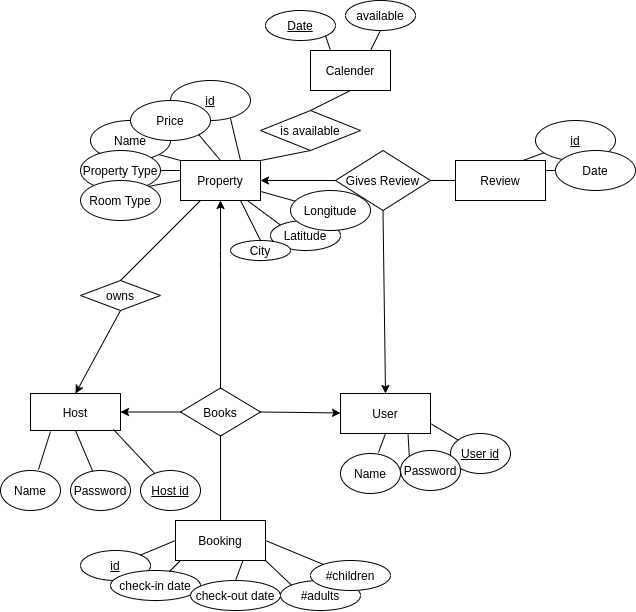
\includegraphics[scale=0.8]{er_diagram.png} 
\caption{ER Diagram for PayRental Service }
\end{figure}

\end{document}
